The goal of this experiment is to study different techniques of AM modulation.

In the first part of the experiment, amplitude modulation will be investigated. The properties of double-sideband modulation and double sideband, supressed carrier modulation, single-sideband modulation and the frequency spectra will be investigated, where the oscilloscope will be used practically to view the effect that changing modulation parameters has on the modulated signal.

The reason signals are modulated is because of the attenuation that signals undergo when going through a medium like air, where low frequency signals are highly attenuated while high frequency signals are attenuated significantly less.

The second reason is because the size of the antenna required to receive a signal is inversely proportional to the frequency. The higher the frequency, the smaller the antenna can be when receiving the signal.

Finally, multiple signals must be transmitted simultaneously. Frequencies that matter to humans are between a few hertz to a few thousand hertz, so modulation is necessary as to not exhaust the available bandwidth.

\section{Band-Limited Signal AM Modulation}
For a sinusoidal carrier signal,
\begin{equation}
    c(t) = A_c \cos(\omega_ct + \phi_c)
\end{equation}

Where for convenience, $\phi_c = 0$. Consider a signal $x(t)$. The {\bf amplitude modulated} signal can now be described by,

\begin{equation}
    y(t) = (1 + kx(t)) \cdot c(t) = A_c\left[1 + kx(t)\right]cos(\omega_ct)
\end{equation}

Where $k$ is defined as the transmitter sensitivity. The expression $kx(t)$ must always be less than unity, otherwise the carrier signal becomes overmodulated and the signal is distorted.

The carrier signal's maximum frequency must also be greater than the maximum frequency of the modulating signal: $f_c \gg f_m$, otherwise an envelope may not be observed.

A band-limited signal is defined as any signal whose frequency spectrum goes to zero outside of a certain range, thereby
\begin{equation}
    X(\omega) = 0 \quad \text{for} \quad |\omega| > \omega_m
\end{equation}

\begin{figure}[H]
    \centering
    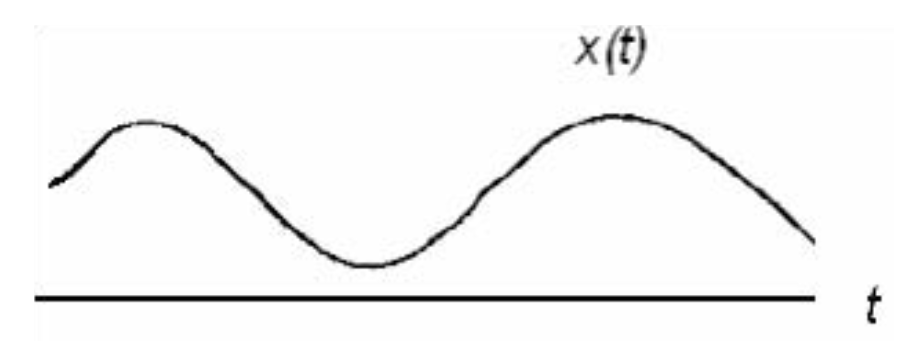
\includegraphics[width=0.5\textwidth]{images/intro_bandlimited_signal_time.png}
    \caption{Time domain representation of a band-limited signal}
    \label{fig:intro_bandlimited_signal_time}
\end{figure}
\begin{figure}[H]
    \centering
    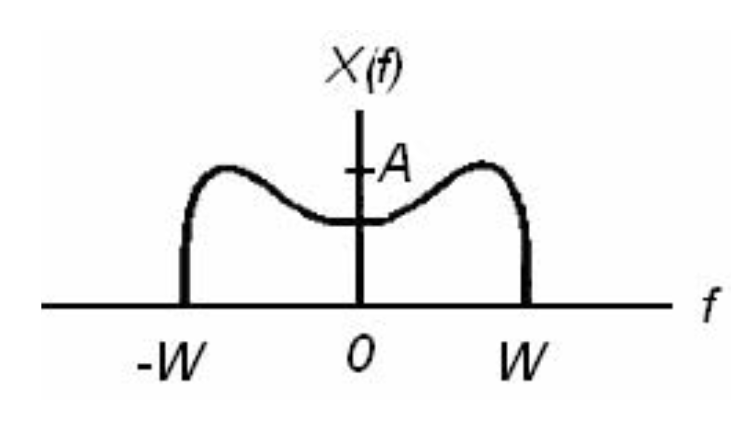
\includegraphics[width=0.5\textwidth]{images/intro_bandlimited_signal.png}
    \caption{Frequency domain representation of a band-limited signal}
    \label{fig:intro_bandlimited_signal_freq}
\end{figure}

And this signal, when modulated, gives the following figure:
\begin{figure}[H]
    \centering
    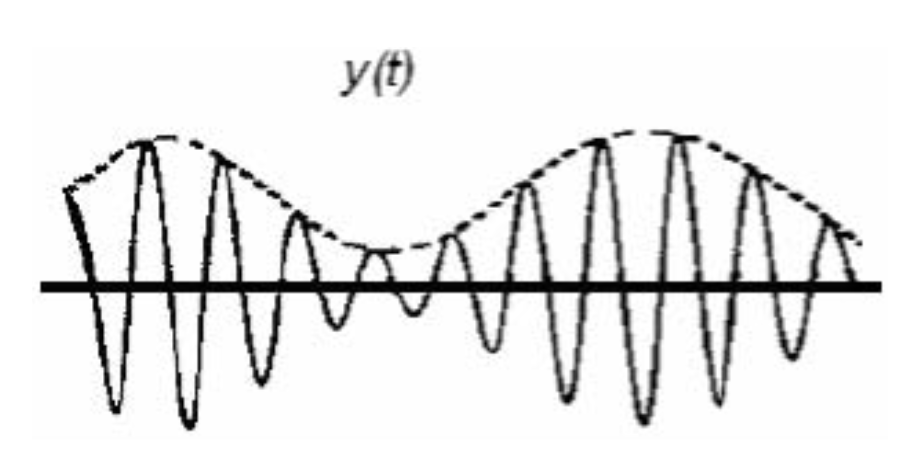
\includegraphics[width=0.5\textwidth]{images/intro_modulated_signal.png}
    \caption{Time domain representation of the modulated signal}
    \label{fig:intro_modulated_signal}
\end{figure}

In the case when $x(t)$ is a sinusoid with a single frequency, the modulated signal can be represented as,

\begin{equation}
    y(t) = A_c\left[1 + kA_m\cos(\omega_mt)\right]\cos(\omega_ct)
\end{equation}

Where $kA_m$ can be written as $m$, the modulation index. The modulation index must be kept below unity, as to not overmodulate the signal.

The frequency spectrum of this function contains deltas, as given by:
\begin{equation}
    \begin{gathered}
        Y(f) = \frac{A_c}{2}\left[\delta(f - f_c) + \delta(f + f_c)\right] \\
        + \frac{mA_c}{4}\left[\delta(f - f_m - f_c) + \delta(f + f_m + f_c)\right] \\
        + \frac{mA_c}{4}\left[\delta(f - f_m + f_c) + \delta(f + f_m - f_c)\right]
    \end{gathered}
\end{equation}

\section{Demodulation Techniques}
For a double-sideband supressed carrier signal, multiplying the modulated signal with the carrier signal will give the original signal back, albeit with a smaller amplitude,

\begin{equation}
    \begin{gathered}
        y(t) = x(t) \cos(\omega_ct) \cdot \cos(\omega_ct) \\
        = x(t) \cos^2(\omega_ct) \\
        = \frac{1}{2}x(t) + \frac{1}{2}x(t)\cos(2\omega_ct)
    \end{gathered}
\end{equation}

Which is obtained using the trigonometric identity,
\begin{equation}
    \cos(\omega_ct)^2 = \frac{1}{2} + \frac{1}{2}\cos(2\omega_ct)
\end{equation}


By applying a low pass filter to the signal, the $\frac{1}{2}x(t)$ term can be kept, while removing the sinusoidal term, recovering the original signal, although with a smaller amplitude.

This is, however, highly ideal. This requires that there is no phase difference between the carrier and the demodulating signal, besides the fact that they must have the same frequency. This is difficult to implement in practice, so another method that can be used is asynchronous detection.

In {\bf asynchronous} detection, the signal is shifted upward by a DC component, such that:
\begin{equation}
    x_c(t) = x(t) + C
\end{equation}

The signal's fourier transform will then have another delta, which represents an inefficiency in the power draw, however, a simple envelope detector can then be used to recover the original signal.

\begin{figure}[H]
    \centering
    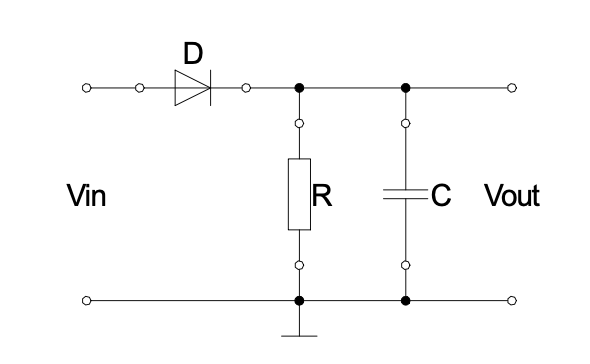
\includegraphics[width=0.5\textwidth]{images/intro_envelope_detector.png}
    \caption{Envelope detector}
    \label{fig:intro_envelope_detector}
\end{figure}

The envelope detector works by the diode allowing only positive voltages to pass through, and the capacitor and resistor are responsible for extracting the shape or the envelope of the signal.